\begin{figure}[t]
  \hspace{0.05\textwidth}%
  \begin{subfigure}[b]{\textwidth}
    \tikzstyle{legend-point}=[circle, inner sep=1.25pt]
    \definecolor{GraphBlue}{HTML}{6c8abd}
    \definecolor{GraphGreen}{HTML}{73b584}
    \definecolor{GraphRed}{HTML}{d07175}
    \definecolor{GraphPurple}{HTML}{8172b2}
    \definecolor{GraphYellow}{HTML}{ccb974}
    
    \definecolor{legend1}{HTML}{eed0cd}
    \definecolor{legend2}{HTML}{deb1d4}
    \definecolor{legend3}{HTML}{aca3d8}
    \definecolor{legend4}{HTML}{72a2b5}
    \definecolor{legend5}{HTML}{549874}
    \definecolor{legend6}{HTML}{5d773b}
    \definecolor{legend7}{HTML}{6c4c2e}
    \definecolor{legend8}{HTML}{5c2b3d}
    \definecolor{legend9}{HTML}{311c3b}
    
    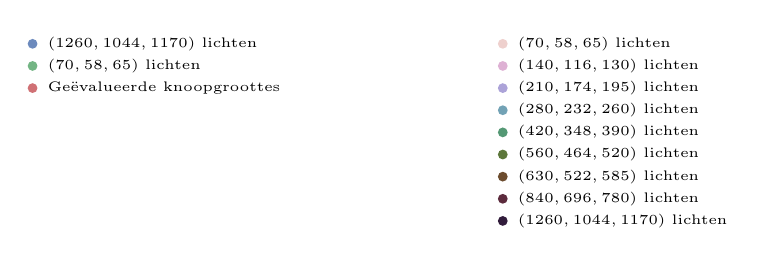
\begin{tikzpicture}
      \node (legend1) at (0.5925\textwidth, 0)
            [legend-point, fill={legend1}, label=right:{\tiny $(70, 58, 65)$  lichten}] {};
      \node (legend2) at (0.5925\textwidth, -8pt)
            [legend-point, fill={legend2}, label=right:{\tiny $(140, 116, 130)$  lichten}] {};
      \node (legend3) at (0.5925\textwidth, -16pt)
            [legend-point, fill={legend3}, label=right:{\tiny $(210, 174, 195)$  lichten}] {};
      \node (legend4) at (0.5925\textwidth, -24pt)
            [legend-point, fill={legend4}, label=right:{\tiny $(280, 232, 260)$  lichten}] {};
      \node (legend5) at (0.5925\textwidth, -32pt)
            [legend-point, fill={legend5}, label=right:{\tiny $(420, 348, 390)$  lichten}] {};
      \node (legend6) at (0.5925\textwidth, -40pt)
            [legend-point, fill={legend6}, label=right:{\tiny $(560, 464, 520)$  lichten}] {};
      \node (legend7) at (0.5925\textwidth, -48pt)
            [legend-point, fill={legend7}, label=right:{\tiny $(630, 522, 585)$  lichten}] {};
      \node (legend8) at (0.5925\textwidth, -56pt)
            [legend-point, fill={legend8}, label=right:{\tiny $(840, 696, 780)$  lichten}] {};
      \node (legend9) at (0.5925\textwidth, -64pt)
            [legend-point, fill={legend9}, label=right:{\tiny $(1260, 1044, 1170)$  lichten}] {};

      \node (legend:naive) at (0.1\textwidth,0)
            [legend-point, fill={GraphBlue}, label=right:{\tiny $(1260, 1044, 1170)$  lichten}] {};
      \node (legend:grid) at (0.1\textwidth, -8pt)
            [legend-point, fill={GraphGreen}, label=right:{\tiny $(70, 58, 65)$ lichten}] {};
      \node (legend:tiled) at (0.1\textwidth, -16pt)
            [legend-point, fill={GraphRed}, label=right:{\tiny Ge\"evalueerde knoopgroottes}] {};
    \end{tikzpicture}
  \end{subfigure}\hfill\\
  \begin{adjustbox}{minipage=\textwidth, scale=0.55}
    \begin{subfigure}[b]{0.8\textwidth}
      \centering
      \def\svgwidth{\textwidth}
      \input{./img/raw/hs-layered-mem/layered_spaceship-indoor_1260_octree.pdf_tex}
      \caption{Spaceship indoor - octree}
      \vspace{4pt}
      \label{fig:hs-layered-mem:indoor-octree}
    \end{subfigure}
  \end{adjustbox} %
  %
  \begin{adjustbox}{minipage=\textwidth, scale=0.55}
    \begin{subfigure}[b]{0.8\textwidth}
      \centering
      \def\svgwidth{\textwidth}
      \input{./img/raw/hs-layered-mem/layered_spaceship-indoor_1260_data.pdf_tex}
      \caption{Spaceship indoor - data}
      \vspace{4pt}
      \label{fig:hs-layered-mem:indoor-data}
    \end{subfigure}
  \end{adjustbox} \\
  %
  \begin{adjustbox}{minipage=\textwidth, scale=0.55}
    \begin{subfigure}[b]{0.8\textwidth}
      \centering
      \def\svgwidth{\textwidth}
      \input{./img/raw/hs-layered-mem/layered_pipers-alley_1044_octree.pdf_tex}
      \caption{Pipers Alley - octree}
      \label{fig:hs-layered-mem:alley-octree}
    \end{subfigure}
  \end{adjustbox}
  %
  \begin{adjustbox}{minipage=\textwidth, scale=0.55}
    \begin{subfigure}[b]{0.8\textwidth}
      \centering
      \def\svgwidth{\textwidth}
      \input{./img/raw/hs-layered-mem/layered_pipers-alley_1044_data.pdf_tex}
      \caption{Pipers Alley - data}
      \label{fig:hs-layered-mem:alley-data}
    \end{subfigure}
  \end{adjustbox} \\
  %
  \begin{adjustbox}{minipage=\textwidth, scale=0.55}
    \begin{subfigure}[b]{0.8\textwidth}
      \centering
      \def\svgwidth{\textwidth}
      \input{./img/raw/hs-layered-mem/layered_ziggurat-city_1170_octree.pdf_tex}
      \caption{Ziggurat City - octree}
      \label{fig:hs-layered-mem:city-octree}
    \end{subfigure}
  \end{adjustbox} %
  %
  \begin{adjustbox}{minipage=\textwidth, scale=0.55}
    \begin{subfigure}[b]{0.8\textwidth}
      \centering
      \def\svgwidth{\textwidth}
      \input{./img/raw/hs-layered-mem/layered_ziggurat-city_1170_data.pdf_tex}
      \caption{Ziggurat city - data}
      \label{fig:hs-layered-mem:city-data}
    \end{subfigure}
  \end{adjustbox}
  \caption{\small Geheugen gebruik per laag van de Hashed Shading datastructuren als functie van de knoopgrootte.}
  \label{fig:hs-layered-mem}
\end{figure}

